\begin{table}[H]
\centering
\definecolor{tabglobalgeneralothernorm0}{rgb}{0.8072,0.0452,0.1316}
\definecolor{tabglobalgeneralothernorm1}{rgb}{0.7792,0.026,0.139}
\definecolor{tabglobalgeneralothernorm2}{rgb}{0.7885,0.0324,0.1366}
\definecolor{tabglobalgeneralothernorm3}{rgb}{0.6821,0.0,0.149}
\definecolor{tabglobalgeneralothernorm4}{rgb}{0.7651,0.0164,0.1427}
\definecolor{tabglobalgeneralothernorm5}{rgb}{0.502,0.0,0.149}
\definecolor{tabglobalgeneralothernorm6}{rgb}{0.6896,0.0,0.149}
\definecolor{tabglobalgeneralothernorm7}{rgb}{0.7698,0.0196,0.1415}
\definecolor{tabglobalgeneralothernorm8}{rgb}{0.8353,0.0644,0.1243}
\definecolor{tabglobalgeneralothernorm9}{rgb}{0.9248,0.1739,0.1292}
\definecolor{tabglobalgeneralothernorm10}{rgb}{0.9309,0.1867,0.1326}
\definecolor{tabglobalgeneralothernorm11}{rgb}{0.9899,0.4096,0.1943}
\definecolor{tabglobalgeneralothernorm12}{rgb}{0.9948,0.6508,0.2776}
\definecolor{tabglobalgeneralothernorm13}{rgb}{0.995,0.6599,0.2816}
\definecolor{tabglobalgeneralothernorm14}{rgb}{0.9896,0.394,0.1899}
\definecolor{tabglobalgeneralothernorm15}{rgb}{0.9949,0.6554,0.2796}
\definecolor{tabglobalgeneralothernorm16}{rgb}{0.9947,0.6463,0.2756}
\definecolor{tabglobalgeneralothernorm17}{rgb}{1.0,0.9801,0.7513}
\definecolor{tabglobalgeneralothernorm18}{rgb}{1.0,0.9402,0.6538}
\definecolor{tabglobalgeneralothernorm19}{rgb}{0.9984,0.8971,0.5596}
\definecolor{tabglobalgeneralothernorm20}{rgb}{0.9961,0.8498,0.4615}
\definecolor{tabglobalgeneralothernorm21}{rgb}{0.9961,0.7634,0.3684}
\definecolor{tabglobalgeneralothernorm22}{rgb}{0.9955,0.6781,0.2894}
\definecolor{tabglobalgeneralothernorm23}{rgb}{0.9933,0.5962,0.254}
\definecolor{tabglobalgeneralothernorm24}{rgb}{0.991,0.4793,0.2143}
\definecolor{tabglobalgeneralothernorm25}{rgb}{0.9888,0.3398,0.1744}
\definecolor{tabglobalgeneralothernorm26}{rgb}{0.9463,0.2187,0.1412}
\definecolor{tabglobalgeneralothernorm27}{rgb}{0.8867,0.0996,0.1107}
\definecolor{tabglobalgeneralothernorm28}{rgb}{0.8025,0.042,0.1329}
\definecolor{tabglobalgeneralothernorm29}{rgb}{0.7046,0.0,0.149}
\definecolor{tabglobalgeneralothernorm30}{rgb}{0.5695,0.0,0.149}
\begin{minipage}{0.78\textwidth}
\centering
\renewcommand{\arraystretch}{1.2}
\begin{tabular}{lccc}
\toprule
Checkpoint & First & Middle & Last \\
\midrule
0 & \cellcolor{tabglobalgeneralothernorm0}\textcolor{white}{$0.408 \pm 0.047$} & \cellcolor{tabglobalgeneralothernorm1}\textcolor{white}{$0.419 \pm 0.062$} & \cellcolor{tabglobalgeneralothernorm1}\textcolor{white}{$0.420 \pm 0.052$} \\
1 & \cellcolor{tabglobalgeneralothernorm2}\textcolor{white}{$0.416 \pm 0.051$} & \cellcolor{tabglobalgeneralothernorm3}\textcolor{white}{$0.452 \pm 0.066$} & \cellcolor{tabglobalgeneralothernorm4}\textcolor{white}{$0.425 \pm 0.057$} \\
5 & \cellcolor{tabglobalgeneralothernorm3}\textcolor{white}{$0.450 \pm 0.050$} & \cellcolor{tabglobalgeneralothernorm5}\textcolor{white}{$0.499 \pm 0.068$} & \cellcolor{tabglobalgeneralothernorm6}\textcolor{white}{$0.448 \pm 0.063$} \\
15 & \cellcolor{tabglobalgeneralothernorm7}\textcolor{white}{$0.424 \pm 0.053$} & \cellcolor{tabglobalgeneralothernorm1}\textcolor{white}{$0.420 \pm 0.070$} & \cellcolor{tabglobalgeneralothernorm8}\textcolor{white}{$0.398 \pm 0.075$} \\
50 & \cellcolor{tabglobalgeneralothernorm9}\textcolor{white}{$0.352 \pm 0.060$} & \cellcolor{tabglobalgeneralothernorm10}\textcolor{white}{$0.348 \pm 0.098$} & \cellcolor{tabglobalgeneralothernorm9}\textcolor{white}{$0.351 \pm 0.073$} \\
200 & \cellcolor{tabglobalgeneralothernorm11}\textcolor{black}{$0.287 \pm 0.058$} & \cellcolor{tabglobalgeneralothernorm12}\textcolor{black}{$0.207 \pm 0.070$} & \cellcolor{tabglobalgeneralothernorm13}\textcolor{black}{$0.203 \pm 0.034$} \\
last & \cellcolor{tabglobalgeneralothernorm14}\textcolor{black}{$0.290 \pm 0.059$} & \cellcolor{tabglobalgeneralothernorm15}\textcolor{black}{$0.205 \pm 0.069$} & \cellcolor{tabglobalgeneralothernorm16}\textcolor{black}{$0.209 \pm 0.032$} \\
\bottomrule
\end{tabular}
\end{minipage}%
\hfill
\begin{minipage}{0.15\textwidth}
\centering
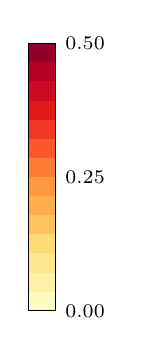
\begin{tikzpicture}
\fill[tabglobalgeneralothernorm17] (0,0.0000) rectangle (0.35,0.2429);
\fill[tabglobalgeneralothernorm18] (0,0.2429) rectangle (0.35,0.4857);
\fill[tabglobalgeneralothernorm19] (0,0.4857) rectangle (0.35,0.7286);
\fill[tabglobalgeneralothernorm20] (0,0.7286) rectangle (0.35,0.9714);
\fill[tabglobalgeneralothernorm21] (0,0.9714) rectangle (0.35,1.2143);
\fill[tabglobalgeneralothernorm22] (0,1.2143) rectangle (0.35,1.4571);
\fill[tabglobalgeneralothernorm23] (0,1.4571) rectangle (0.35,1.7000);
\fill[tabglobalgeneralothernorm24] (0,1.7000) rectangle (0.35,1.9429);
\fill[tabglobalgeneralothernorm25] (0,1.9429) rectangle (0.35,2.1857);
\fill[tabglobalgeneralothernorm26] (0,2.1857) rectangle (0.35,2.4286);
\fill[tabglobalgeneralothernorm27] (0,2.4286) rectangle (0.35,2.6714);
\fill[tabglobalgeneralothernorm28] (0,2.6714) rectangle (0.35,2.9143);
\fill[tabglobalgeneralothernorm29] (0,2.9143) rectangle (0.35,3.1571);
\fill[tabglobalgeneralothernorm30] (0,3.1571) rectangle (0.35,3.4000);
\draw[black,line width=0.3pt] (0,0) rectangle (0.35,3.4000);
\node[right,font=\scriptsize,anchor=west] at (0.35,3.4000) {0.50};
\node[right,font=\scriptsize,anchor=west] at (0.35,1.7000) {0.25};
\node[right,font=\scriptsize,anchor=west] at (0.35,0) {0.00};
\end{tikzpicture}
\end{minipage}
\caption{Global Wasserstein alignment, GeneralSheaf other Laplacian: maps trained \texttt{norm=False}, evaluated normalised. Mean $\pm$ SE across 10 datasets (First/Last), 8 for Middle (datasets with $L=2$ contribute no middle layer). (Pooled fold/layer SE averages 0.017 across cells; not shown per cell, see text.) Cell shading: white = 0, dark red = 0.50 (max value in this table), YlOrRd colormap, same scale as Fig.~\ref{fig: RM_Norm} etc.}
\label{tab:global_general_other_norm}
\end{table}
